\documentclass[tikz,border=10pt]{standalone}
\usepackage{tikz}
\usetikzlibrary{matrix}

\tikzset{
  cell/.style={draw=black!70, line width=1.0pt, minimum width=5.1cm, minimum height=1.25cm, align=center, text width=4.7cm, fill=none},
  head/.style={cell, draw=blue!70!black, line width=1.2pt}
}

\begin{document}
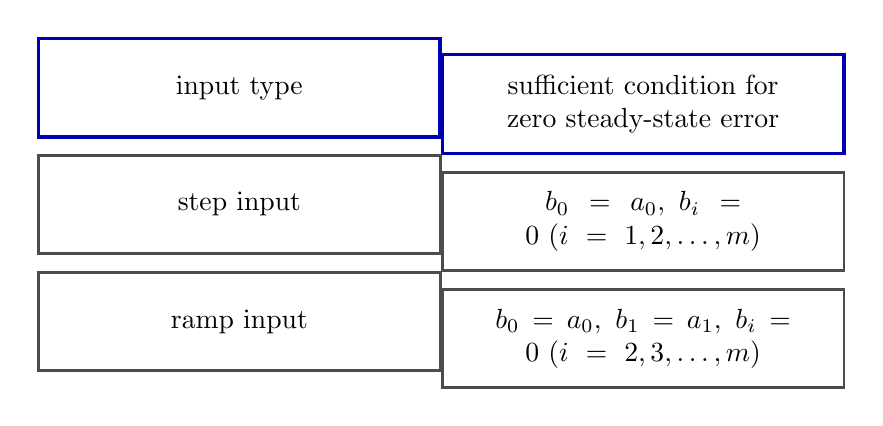
\begin{tikzpicture}
  \matrix[matrix of nodes, nodes in empty cells, row sep=-\pgflinewidth, column sep=-\pgflinewidth] {
    \node[head] {input type}; &
    \node[head] {sufficient condition for zero steady-state error}; \\
    \node[cell] {step input}; &
    \node[cell] {$b_0=a_0,\ b_i=0\ (i=1,2,\dots,m)$}; \\
    \node[cell] {ramp input}; &
    \node[cell] {$b_0=a_0,\ b_1=a_1,\ b_i=0\ (i=2,3,\dots,m)$}; \\
  };
\end{tikzpicture}
\end{document}
